\documentclass[border=8pt]{standalone}
\usepackage{fontspec}
\IfFileExists{fonts/times.ttf}{
  \setmainfont{times.ttf}[Path=fonts/,
    BoldFont=timesbd.ttf, ItalicFont=timesi.ttf, BoldItalicFont=timesbi.ttf]
}{\usepackage{mathptmx}}
\usepackage{tikz}
\usetikzlibrary{arrows.meta,positioning,calc}
\begin{document}
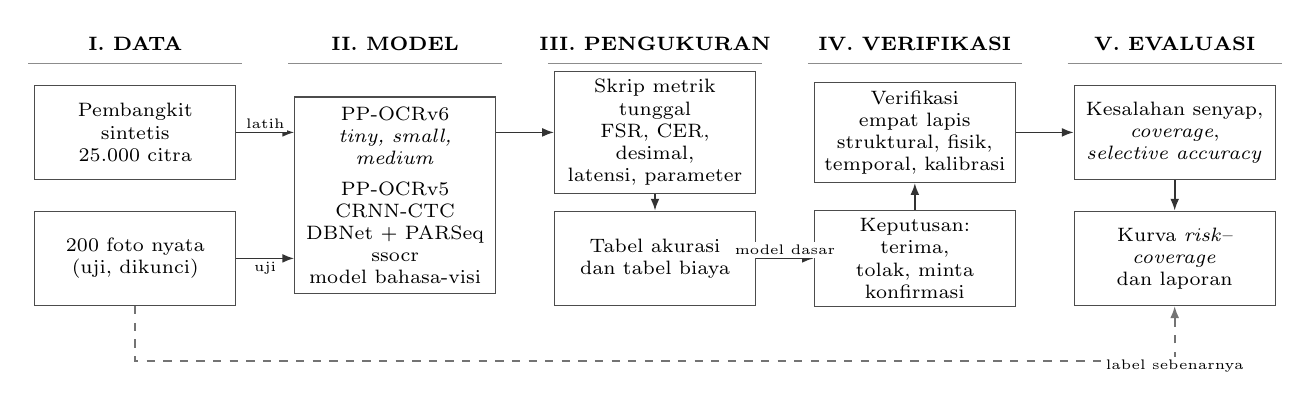
\begin{tikzpicture}[
  x=1cm, y=1cm,
  kotak/.style={rectangle, draw=black!70, fill=white, align=center,
                text width=2.34cm, inner sep=3pt, font=\scriptsize},
  tahap/.style={font=\scriptsize\bfseries, anchor=south},
  lbl/.style={font=\tiny, align=center, inner sep=1pt, fill=white},
  panah/.style={-{Latex[length=1.5mm]}, draw=black!80, semithick}
]

% ---------------- kepala tahap ----------------
\foreach \x/\nm in {1.55/I. DATA, 4.85/II. MODEL, 8.15/III. PENGUKURAN,
                    11.45/IV. VERIFIKASI, 14.75/V. EVALUASI}{
  \node[tahap] at (\x,1.22) {\nm};
  \draw[black!45] (\x-1.36,1.18) -- (\x+1.36,1.18);
}

% ---------------- I. DATA ----------------
\node[kotak, minimum height=1.20cm] (latih) at (1.55,0.30)
  {Pembangkit sintetis\\ 25.000 citra};
\node[kotak, minimum height=1.20cm] (uji) at (1.55,-1.30)
  {200 foto nyata\\ (uji, dikunci)};

% ---------------- II. MODEL ----------------
\node[kotak, minimum height=2.50cm] (model) at (4.85,-0.50)
  {PP-OCRv6\\ \textit{tiny, small, medium}\\[3pt]
   PP-OCRv5\\ CRNN-CTC\\ DBNet + PARSeq\\ ssocr\\ model bahasa-visi};

% ---------------- III. PENGUKURAN ----------------
\node[kotak, minimum height=1.20cm] (metrik) at (8.15,0.30)
  {Skrip metrik tunggal\\ FSR, CER, desimal,\\ latensi, parameter};
\node[kotak, minimum height=1.20cm] (tabel) at (8.15,-1.30)
  {Tabel akurasi\\ dan tabel biaya};

% ---------------- IV. VERIFIKASI ----------------
\node[kotak, minimum height=1.20cm] (verif) at (11.45,0.30)
  {Verifikasi empat lapis\\ struktural, fisik,\\ temporal, kalibrasi};
\node[kotak, minimum height=1.20cm] (putus) at (11.45,-1.30)
  {Keputusan: terima,\\ tolak, minta konfirmasi};

% ---------------- V. EVALUASI ----------------
\node[kotak, minimum height=1.20cm] (nilai) at (14.75,0.30)
  {Kesalahan senyap,\\ \textit{coverage},\\ \textit{selective accuracy}};
\node[kotak, minimum height=1.20cm] (lapor) at (14.75,-1.30)
  {Kurva \textit{risk--coverage}\\ dan laporan};

% ---------------- panah ----------------
\draw[panah] (latih.east) -- node[lbl, above] {latih} (model.west |- latih.east);
\draw[panah] (uji.east) -- node[lbl, below] {uji} (model.west |- uji.east);
\draw[panah] (model.east |- metrik.east) -- (metrik.west);
\draw[panah] (metrik) -- (tabel);
\draw[panah] (tabel.east) -- node[lbl, above] {model dasar} (putus.west);
\draw[panah] (putus) -- (verif);
\draw[panah] (verif.east) -- (nilai.west);
\draw[panah] (nilai) -- (lapor);
\draw[panah, dashed, draw=black!55] (uji.south) -- ++(0,-0.70) -|
  node[lbl, below, pos=0.55] {label sebenarnya} (lapor.south);

\end{tikzpicture}
\end{document}
